\begin{definition}[צפיפות]
\emph{צפיפות}
של גרף לא מכוון, 
$G = (V, E)$, 
היא 
$\frac{|E|}{|V|}$.
\end{definition}
בהינתן גרף לא מכוון רוצים למצוא תת-גרף שלו צפוף ביותר. מה תת גרף כזה מייצג ברשת חברתית למשל?

\begin{example}
מהי הצפיפות של הגרף הבא? מה התת-גרף הצפוף ביותר של הגרף הבא?
\end{example}

\begin{center}
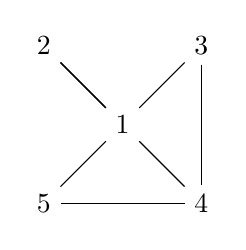
\begin{tikzpicture}
\foreach[count=\i] \x \y in{
	0/0, -1/1, 1/1, 1/-1, -1/-1%
}{
	\node(\i) at(\x,\y) {\i};
}

\foreach \u \v in{
	1/5, 1/4, 4/5, 1/2, 1/3, 3/4, 1/2%
}{
	\draw (\u) -- (\v);
}
\end{tikzpicture}
\end{center}

\textbf{מציאת תת גרף צפוף ביותר על ידי חתך מינימום}

בהינתן גרף לא מכוון, 
$G = (V, E)$, 
נבנה את רשת הזרימה 
$N = (D, s, t, c)$
כאשר 
$D = (\{s,t\} \cup V, s \times V \cup \{uv, vu : uv \in E\}, V \times t)$ 
ואת $c$ נגדיר בהמשך.

\begin{example}
עבור הגרף מהדוגמה הקודמת, רשת הזרימה המתאימה היא:
\end{example}

\begin{center}
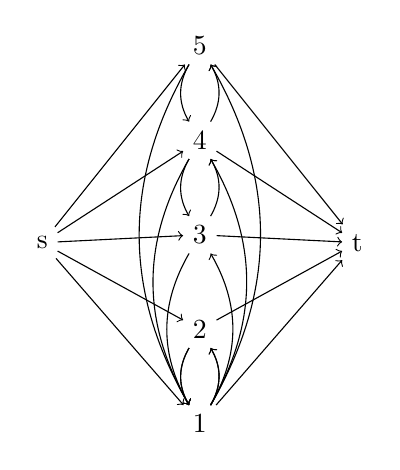
\begin{tikzpicture}

% NODES
\node(s) at(0, 0) {s};

\begin{scope}[y=1.2cm, yshift=-3.5cm]
\foreach \i in{1,...,5}{
	\node(\i) at(2,\i) {\i};
}
\end{scope}

\node(t) at(4, 0) {t};

% ARCS
\foreach \i in{1,...,5}{
	\draw[->] (s) -- (\i);
}

\foreach \u \v in{
	1/5, 1/4, 4/5, 1/2, 1/3, 3/4, 1/2%
}{
	\draw[->] (\u) to[bend right] (\v);
	\draw[->] (\v) to[bend right] (\u);
}

\foreach \i in{1,...,5}{
	\draw[->] (\i) -- (t);
}

\end{tikzpicture}
\end{center}


עבור $x$ כלשהו נגדיר את פונקציית הקיבול להיות
$$
\begin{array}{ll}
\forall \; i 		& c(s, i) = m
\\
\forall \; i		& c(i, t) = m + x - d_G(i)
\\
\forall \; uv \in E	& c(u, v) = 1
\end{array}
$$

עבור תת קבוצה של צמתים,  
$S \subseteq V$, 
מה הערך של 
\stcut{} $\{s\} \cup S$?

\begin{center}
\begin{tikzpicture}

% NODES
\node(s) at(0, 0) {s};

\node(1) 			at(4, 2) {1};
\node[draw=none] 	at(4, 1) {$\vdots$};
\node(i) 			at(4, 0) {i};
\node[draw=none] 	at(4, -1) {$\vdots$};
\node(n) 			at(4, -2) {n};

\node(t) at(8, 0) {t};

% ARCS
\draw[->] (s) -- (1) node[label inside] {m};
\draw[->] (s) -- (i) node[label inside] {m};
\draw[->] (s) -- (n) node[label inside] {m};
%
\draw[->] (1) -- (t) node[label inside] {$m + x - d_G(1)$};
\draw[->] (i) -- (t) node[label inside] {$m + x - d_G(i)$};
\draw[->] (n) -- (t) node[label inside] {$m + x - d_G(n)$};


% CUT
\draw[orange, dashed, very thick]
(s.west)	to[out=90, in=180]
(1.north)	to[out=0, in=90]
(i.east)	to[out=-90, in=-90]
(s.west)
;
\end{tikzpicture}
\end{center}

נסמן ב-
$D(S) \defeq \frac{|E \cap (S \times S)|}{|S|}$ 
את הצפיפות של הגרף המושרה 
$G[S]$.

אז אפשר להשתכנע שקיבול החתך 
$\{s\} \cup S$ 
הוא
$nm + |S|(x - 2D(S))$.

נסמן ב-%
$S^*$ 
קבוצת צמתים כך של-%
$G[S^*]$ 
צפיפות מקסימלית.
\begin{claim}
עבור ערך 
$x < 2D(S^*)$ 
מתקיים שקיבול חתך מינימום ברשת הזרימה הנ"ל קטן מ-
$nm$.
\end{claim}

\begin{proof}
נובע מכך שקיבול החתך 
$\{s\} \cup S^*$
קטן מ-%
$mn$.
\end{proof}

\begin{claim}
עבור ערך 
$x > 2D(S^*)$ 
מתקיים שקיבול חתך מינימום ברשת הזרימה הנ"ל גדול או שווה ל-
$nm$.
\end{claim}

\begin{proof}
נובע מכך שהביטוי 
$|S|(x - 2D(S)) \geq 0$ 
לכל 
$S \subseteq V$.
\end{proof}

\begin{claim}
עבור ערך 
$x = 2D(S^*)$ 
מתקיים שקיבול חתך מינימום ברשת הזרימה הנ"ל הוא
$nm$.
\end{claim}

\begin{proof}
נובע מכך שהביטוי 
$|S|(x - 2D(S)) \geq 0$ 
לכל 
$S \subseteq V$
ו-
$|S^*|(x - 2D(S^*)) = 0$.
\end{proof}

\textbf{אלגוריתם:}
מהטענות הנ"ל ומהעובדה שמספר הצפיפויות האפשרויות הוא פולינומי ניתן לגזור את האלגוריתם הבא:

\begin{enumerate}
\item
"נחש" (בצע חיפוש בינרי) ערך $x$ ובדוק שקיים חתך מינימום עם ערך $nm$ שמכיל יותר מצומת אחד, 
$\{s\} \cup S$.
\item
החזר את 
$S$.
\end{enumerate}
